\documentclass[aspectratio=169,11pt]{beamer}

\def\courseTitle{Industrial Security (Bachelor)}
\def\courseSubtitle{Section 03 -- Industrial Network Architectures}
\def\sectionNumber{03}
\def\sectionTitle{Industrial Network Architectures}

% =====================================================================
% Industrial Security lecture series -- modern Beamer preamble.
%
% Each slide deck must define the following BEFORE \input{}-ing this:
%   \def\courseTitle{...}        e.g. Industrial Security (Bachelor)
%   \def\courseSubtitle{...}     e.g. Section 3 -- Network Architecture
%   \def\sectionNumber{...}      e.g. 03
%   \def\sectionTitle{...}       e.g. Industrial Network Architectures
%
% Optional:
%   \def\courseAuthor{...}       defaults to "Lecture Notes"
%   \def\courseInstitute{...}    defaults to "Department of Computer Science"
%   \def\companyLogo{...}        path to a logo image (PDF/PNG/JPG).
%
% Callout macros (use anywhere inside a frame):
%   \begin{notebox}{title}      ... \end{notebox}
%   \begin{importantbox}{title} ... \end{importantbox}
%   \begin{warningbox}{title}   ... \end{warningbox}
%   \begin{tipbox}{title}       ... \end{tipbox}
%   \begin{defbox}{title}       ... \end{defbox}
%   \begin{takeawaybox}{title}  ... \end{takeawaybox}
%   \begin{quotebox}            ... \end{quotebox}
% =====================================================================

% --- Speaker-notes mode (toggled by Makefile via -usepretex) ----------
% When notesmode=1, build a side-by-side slide+notes PDF for the
% lecturer. When unset/0, build the clean slides-only PDF.
\providecommand{\notesmode}{0}
\ifnum\notesmode=1
  \usepackage{pgfpages}
  \setbeameroption{show notes on second screen=right}
  \setbeamerfont{note page}{size=\small}
\fi

\usepackage[utf8]{inputenc}
\usepackage[T1]{fontenc}
\usepackage[english]{babel}
% Modern type pair: IBM Plex Sans for text, IBM Plex Mono for code.
% Math stays in lmodern; Plex is the dominant family on every text frame.
\usepackage{plex-sans}
\usepackage{plex-mono}
\renewcommand{\familydefault}{\sfdefault}
\usepackage[activate={true,nocompatibility},final,tracking=true,kerning=true,spacing=true,factor=1100,stretch=10,shrink=10]{microtype}
\usepackage{graphicx}
\usepackage{listings}
\usepackage{xcolor}
\usepackage{colortbl}
\usepackage{tikz}
\usepackage{booktabs}
\usepackage{array}
\usepackage{hyperref}
\usepackage{amsmath}
\usepackage{amssymb}
\usepackage{tcolorbox}
\tcbuselibrary{skins, breakable, raster}
\usepackage{fontawesome5}

% =====================================================================
% Shared TikZ styles for the Industrial Security lecture series.
% Loaded by every slide deck and exercise sheet that uses TikZ.
% =====================================================================

\usetikzlibrary{
  arrows.meta,
  shapes,
  shapes.geometric,
  shapes.symbols,
  shapes.multipart,
  positioning,
  fit,
  calc,
  backgrounds,
  decorations.pathmorphing,
  decorations.pathreplacing,
  decorations.text,
  patterns,
  matrix,
  shadows
}

% --- colour palette --------------------------------------------------
\definecolor{isOT}{HTML}{1F4E79}     % OT (deep blue)
\definecolor{isIT}{HTML}{6F2DA8}     % IT (purple)
\definecolor{isSafety}{HTML}{C00000} % safety red
\definecolor{isNet}{HTML}{2E7D32}    % network green
\definecolor{isAttack}{HTML}{B23A48} % attack red
\definecolor{isAccent}{HTML}{E08E0B} % amber
\definecolor{isMute}{HTML}{6B6B6B}   % grey
\definecolor{isLight}{HTML}{EDF2F8}  % light background
\definecolor{isPLC}{HTML}{2C5282}
\definecolor{isHMI}{HTML}{2F855A}
\definecolor{isSCADA}{HTML}{6B46C1}

% --- generic node styles --------------------------------------------
\tikzset{
  isnode/.style={
    draw, rounded corners=2pt, minimum height=8mm, minimum width=18mm,
    font=\small, align=center, thick
  },
  isbox/.style={isnode, fill=isLight},
  plc/.style={isnode, fill=isPLC!15, draw=isPLC, thick},
  hmi/.style={isnode, fill=isHMI!15, draw=isHMI, thick},
  scada/.style={isnode, fill=isSCADA!15, draw=isSCADA, thick},
  sensor/.style={isnode, fill=isNet!10, draw=isNet, minimum height=6mm, minimum width=14mm, font=\scriptsize},
  actuator/.style={isnode, fill=isAccent!15, draw=isAccent, minimum height=6mm, minimum width=14mm, font=\scriptsize},
  firewall/.style={isnode, fill=isAttack!15, draw=isAttack, thick},
  server/.style={isnode, fill=isMute!15, draw=isMute!80, thick},
  switch/.style={isnode, fill=isLight, draw=black!60, minimum height=6mm, minimum width=14mm, font=\scriptsize},
  workstation/.style={isnode, fill=white, draw=isOT, thick},
  attacker/.style={isnode, fill=isAttack!20, draw=isAttack, thick, font=\small\bfseries},
  inetnode/.style={draw, ellipse, minimum width=24mm, minimum height=10mm, font=\scriptsize, fill=isLight, thick},
  process/.style={isnode, fill=isOT!15, draw=isOT, thick, minimum width=24mm},
  zone/.style={
    draw, rounded corners=4pt, thick, dashed, inner sep=4mm
  },
  conduit/.style={-{Stealth[length=2.5mm]}, thick, isNet!80!black},
  attack/.style={-{Stealth[length=2.5mm]}, thick, isAttack, dashed},
  flow/.style={-{Stealth[length=2.5mm]}, thick, isOT!70!black},
  netline/.style={thick, black!60},
  axisline/.style={-{Stealth[length=2mm]}, thick, black!70},
  tag/.style={font=\scriptsize\itshape, fill=white, inner sep=1pt},
  level/.style={
    draw, fill=isLight, minimum width=0.85\linewidth, minimum height=8mm,
    font=\small, anchor=west
  },
  brace/.style={decorate, decoration={brace, amplitude=4pt, raise=2pt}},
  legendbox/.style={draw, rounded corners=2pt, fill=isLight, inner sep=2mm, font=\scriptsize, align=left}
}

% --- handy macros ----------------------------------------------------
% \plcicon, \hmiicon etc as simple labelled boxes; useful inline.
\newcommand{\plcicon}[1][PLC]{\tikz[baseline=-0.6ex]{\node[plc, minimum width=10mm, minimum height=5mm, font=\scriptsize, inner sep=1pt]{#1};}}
\newcommand{\hmiicon}[1][HMI]{\tikz[baseline=-0.6ex]{\node[hmi, minimum width=10mm, minimum height=5mm, font=\scriptsize, inner sep=1pt]{#1};}}
\newcommand{\fwicon}[1][FW]{\tikz[baseline=-0.6ex]{\node[firewall, minimum width=10mm, minimum height=5mm, font=\scriptsize, inner sep=1pt]{#1};}}


\graphicspath{{.}{../../../template/}}

% --- defaults --------------------------------------------------------
\providecommand{\courseAuthor}{Lecture Notes}
\providecommand{\courseInstitute}{Department of Computer Science}
\providecommand{\companyLogo}{logo}

% --- modern palette --------------------------------------------------
\definecolor{slideAccent}{HTML}{1F4E79}       % primary navy
\definecolor{slideSecondary}{HTML}{E08E0B}    % amber accent

% --- Corporate branding overrides ------------------------------------
% A user-editable `branding.tex` at the repo root can override the
% logo path, author/institute lines, and brand colours. If the file is
% missing the built-in defaults above stay in effect.
\IfFileExists{../../../branding.tex}{% =====================================================================
% Corporate / institutional branding -- single file to customise the
% look of the entire course (slides, notes, exercises, labs).
%
% HOW TO REBRAND IN UNDER A MINUTE:
%   1. Replace `branding/logo.pdf` with your own logo
%      (PDF preferred; PNG and JPG also work -- name it `logo.<ext>`).
%   2. (Optional) change the two colours below to your brand palette.
%   3. (Optional) override the author/institute lines below.
%   4. Re-run `make` at the repo root. That's it.
%
% Everything in this file has sensible defaults; you can delete a line
% to fall back to the built-in defaults, or comment it out.
%
% This file is loaded automatically by the slides, exercise, and lab
% preambles -- you never need to \input it manually.
% =====================================================================

% --- Logo --------------------------------------------------------------
% Path is resolved from each leaf-build directory; the default points at
% the shared `branding/` folder at the repo root. If you put your logo
% somewhere else, set the full or relative path here (without extension):
\renewcommand{\companyLogo}{../../../branding/logo}

% --- Author / institute (appears on the title page footer) ------------
\renewcommand{\courseAuthor}{}
\renewcommand{\courseInstitute}{}

% --- Brand colours ----------------------------------------------------
% slideAccent      = primary brand colour (title bands, accent rule)
% slideSecondary   = secondary brand colour (section badge, highlight)
% Both use HTML hex codes. Keep enough contrast against white text.
\definecolor{slideAccent}{HTML}{00205B}      % deep navy
\definecolor{slideSecondary}{HTML}{00A0DC}   % light blue accent
}{}
\definecolor{slideTitle}{HTML}{0F2A44}        % near-black navy
\definecolor{slideMuted}{HTML}{6B6B6B}
\definecolor{slideBg}{HTML}{FFFFFF}
\definecolor{slidePanel}{HTML}{F4F7FB}
\definecolor{slideRule}{HTML}{D6DEE8}

% Callout colours
\definecolor{calNote}{HTML}{1F4E79}
\definecolor{calImportant}{HTML}{B23A48}
\definecolor{calWarning}{HTML}{C77700}
\definecolor{calTip}{HTML}{2E7D32}
\definecolor{calDef}{HTML}{6B46C1}
\definecolor{calTake}{HTML}{0F2A44}

% --- beamer theme ---------------------------------------------------
\useinnertheme{rectangles}
\usefonttheme{professionalfonts}

\setbeamertemplate{navigation symbols}{}
\setbeamertemplate{itemize items}[circle]
\setbeamertemplate{enumerate items}[default]
\setbeamertemplate{section in toc}[ball numbered]
\setbeamercolor{section in toc}{fg=slideTitle}

% Colours
\setbeamercolor{normal text}{fg=slideTitle, bg=slideBg}
\setbeamercolor{title}{fg=slideAccent}
\setbeamercolor{subtitle}{fg=slideMuted}
\setbeamercolor{frametitle}{fg=slideAccent}
\setbeamercolor{structure}{fg=slideAccent}
\setbeamercolor{itemize item}{fg=slideAccent}
\setbeamercolor{itemize subitem}{fg=slideSecondary}
\setbeamercolor{block title}{fg=white, bg=slideAccent}
\setbeamercolor{block body}{fg=slideTitle, bg=slidePanel}
\setbeamercolor{alerted text}{fg=slideSecondary}

% Fonts
\setbeamerfont{title}{series=\bfseries, size=\Large}
\setbeamerfont{subtitle}{series=\mdseries, size=\normalsize}
\setbeamerfont{frametitle}{series=\bfseries, size=\large}
\setbeamerfont{block title}{series=\bfseries, size=\normalsize}
\setbeamerfont{footline}{size=\tiny}

% --- frametitle: title bar + accent underline + section badge -------
% The accent rules are wrapped in a zero-width box so they never
% contribute to the surrounding hbox width (no Overfull warnings).
\setbeamertemplate{frametitle}{%
  \nointerlineskip
  \begin{beamercolorbox}[wd=\paperwidth, ht=2.8ex, dp=1.6ex, leftskip=1.2em, rightskip=1.2em]{frametitle}%
    \usebeamerfont{frametitle}\insertframetitle%
    \hfill
    {\color{slideMuted}\small \sectionNumber}%
  \end{beamercolorbox}%
  \nointerlineskip
  \makebox[0pt][l]{\hspace*{1.2em}\textcolor{slideSecondary}{\rule{2.5em}{1pt}}\textcolor{slideAccent}{\rule{\dimexpr\paperwidth-3.7em\relax}{1pt}}}%
  \par\vskip4pt
}

% --- footer ---------------------------------------------------------
\defbeamertemplate*{footline}{is-footer}{%
  \leavevmode%
  \hbox{%
    \begin{beamercolorbox}[wd=.55\paperwidth, ht=2.4ex, dp=1ex, leftskip=1em]{author in head/foot}%
      {\color{slideMuted}\tiny \courseTitle{} \;\; $\bullet$ \;\; Section \sectionNumber{} -- \sectionTitle}%
    \end{beamercolorbox}%
    \begin{beamercolorbox}[wd=.45\paperwidth, ht=2.4ex, dp=1ex, rightskip=1em]{title in head/foot}%
      \hfill {\color{slideMuted}\tiny \insertframenumber{} / \inserttotalframenumber}%
    \end{beamercolorbox}%
  }%
  \vskip2pt
}

% --- listings -------------------------------------------------------
\definecolor{codebg}{HTML}{F4F7FB}
\definecolor{codekw}{HTML}{0F2A44}
\definecolor{codestr}{HTML}{8B3A3A}
\definecolor{codecom}{HTML}{5A7D54}

\lstset{
    backgroundcolor=\color{codebg},
    basicstyle=\ttfamily\scriptsize\color{slideTitle},
    keywordstyle=\color{codekw}\bfseries,
    stringstyle=\color{codestr},
    commentstyle=\color{codecom}\itshape,
    breaklines=true,
    frame=leftline,
    framerule=2pt,
    rulecolor=\color{slideAccent},
    numbers=left,
    numberstyle=\tiny\color{slideMuted},
    numbersep=8pt,
    showstringspaces=false,
    tabsize=2,
    captionpos=b,
    xleftmargin=0.6em
}

% --- callout boxes --------------------------------------------------
% Shared base style for all callout boxes.
% Subtle drop shadow gives the boxes a hint of elevation without distraction.
\tcbset{
  isCallout/.style={
    enhanced, breakable, sharp corners=northeast,
    arc=2pt, boxrule=0pt,
    leftrule=3pt,
    fonttitle=\bfseries\small,
    coltitle=white,
    fontupper=\small,
    left=2mm, right=2mm, top=1.5mm, bottom=1.5mm,
    drop fuzzy shadow=black!30,
    title={#1}
  }
}

\newtcolorbox{notebox}[1]{
  isCallout={#1},
  colback=calNote!8, colframe=calNote, leftrule=3pt,
  colbacktitle=calNote, attach boxed title to top left={xshift=2mm, yshift=-1.2mm},
  boxed title style={colback=calNote, arc=1pt, boxrule=0pt, left=2mm, right=2mm, top=0.5mm, bottom=0.5mm}
}

\newtcolorbox{importantbox}[1]{
  isCallout={#1},
  colback=calImportant!7, colframe=calImportant, leftrule=4pt,
  colbacktitle=calImportant, attach boxed title to top left={xshift=2mm, yshift=-1.2mm},
  boxed title style={colback=calImportant, arc=1pt, boxrule=0pt, left=2mm, right=2mm, top=0.5mm, bottom=0.5mm}
}

\newtcolorbox{warningbox}[1]{
  isCallout={#1},
  colback=calWarning!10, colframe=calWarning, leftrule=4pt,
  colbacktitle=calWarning, attach boxed title to top left={xshift=2mm, yshift=-1.2mm},
  boxed title style={colback=calWarning, arc=1pt, boxrule=0pt, left=2mm, right=2mm, top=0.5mm, bottom=0.5mm}
}

% Alias warnbox = warningbox, with an optional title (default = "Caution")
\newtcolorbox{warnbox}[1][Caution]{
  isCallout={#1},
  colback=calWarning!10, colframe=calWarning, leftrule=4pt,
  colbacktitle=calWarning, attach boxed title to top left={xshift=2mm, yshift=-1.2mm},
  boxed title style={colback=calWarning, arc=1pt, boxrule=0pt, left=2mm, right=2mm, top=0.5mm, bottom=0.5mm}
}

\newtcolorbox{tipbox}[1]{
  isCallout={#1},
  colback=calTip!8, colframe=calTip, leftrule=3pt,
  colbacktitle=calTip, attach boxed title to top left={xshift=2mm, yshift=-1.2mm},
  boxed title style={colback=calTip, arc=1pt, boxrule=0pt, left=2mm, right=2mm, top=0.5mm, bottom=0.5mm}
}

\newtcolorbox{defbox}[1]{
  isCallout={#1},
  colback=calDef!8, colframe=calDef, leftrule=3pt,
  colbacktitle=calDef, attach boxed title to top left={xshift=2mm, yshift=-1.2mm},
  boxed title style={colback=calDef, arc=1pt, boxrule=0pt, left=2mm, right=2mm, top=0.5mm, bottom=0.5mm}
}

\newtcolorbox{takeawaybox}[1]{
  enhanced, breakable, arc=3pt, boxrule=0pt,
  colback=calTake!7, colframe=calTake,
  toptitle=2mm, bottomtitle=2mm,
  fonttitle=\bfseries\normalsize, coltitle=white,
  colbacktitle=calTake,
  fontupper=\small,
  title={\faStar~Key Takeaway: #1},
  left=3mm, right=3mm, top=2mm, bottom=2mm
}

\newtcolorbox{quotebox}{
  enhanced, breakable, arc=2pt, boxrule=0pt,
  colback=slidePanel, colframe=slideMuted,
  leftrule=3pt, top=2mm, bottom=2mm, left=3mm, right=3mm,
  fontupper=\itshape\small,
}

% Convenience: inline highlight badge
\newcommand{\remembertag}{\tikz[baseline=-0.7ex]\node[fill=calImportant, text=white, font=\scriptsize\bfseries, rounded corners=2pt, inner sep=2pt]{REMEMBER};}
\newcommand{\tldr}{\tikz[baseline=-0.7ex]\node[fill=calTake, text=white, font=\scriptsize\bfseries, rounded corners=2pt, inner sep=2pt]{TL;DR};}

% Source attribution: tiny grey line, anchored bottom-left of the content area
% Usage:  \source{Symantec, \emph{W32.Stuxnet Dossier} v1.4, 2011.}
% Multiple sources:  \source{X.\ Y., 2018; Z, 2020.}
\newcommand{\source}[1]{%
  \par\nointerlineskip\vspace{0.4mm}%
  {\color{slideMuted}\fontsize{5.5}{6.5}\selectfont\textit{Source:} #1\par}%
}

% References slide: aggregate citations + further reading at the end of a section.
% Usage:  \referencesframe{ \item ... \item ... }
% The `frame` environment must be written literally in the deck, so this is a
% macro rather than a wrapper environment (beamer collects the frame body and
% trips over \newenvironment wrappers).
%
% allowframebreakstemplate=\insertcontinuationcount silences the trailing roman
% numeral when content fits on a single page.
\setbeamertemplate{frametitle continuation}[from second]
\newcommand{\referencesframe}[1]{%
  \begin{frame}[allowframebreaks]{References -- Section \sectionNumber}
    \fontsize{7.5}{9}\selectfont
    \setlength{\itemsep}{1pt}
    \begin{itemize}#1\end{itemize}
  \end{frame}%
}

% --- title page -----------------------------------------------------
\title[\courseTitle]{\courseTitle}
\subtitle{\courseSubtitle}
\author{\courseAuthor}
\institute{\courseInstitute}
\date{}

% Logo lookup: try the section directory, then the shared template/.
\newcommand{\showlogo}[1][2cm]{%
  \IfFileExists{\companyLogo.pdf}{\includegraphics[width=#1]{\companyLogo}}{%
    \IfFileExists{\companyLogo.png}{\includegraphics[width=#1]{\companyLogo}}{%
      \IfFileExists{\companyLogo.jpg}{\includegraphics[width=#1]{\companyLogo}}{%
        \IfFileExists{../../../template/\companyLogo.pdf}{\includegraphics[width=#1]{../../../template/\companyLogo}}{%
          \rule{0pt}{0pt}}}}}}

\setbeamertemplate{title page}{%
  
\begin{tikzpicture}[remember picture, overlay]
    % accent band (taller to fit wrapped titles)
    \fill[slideAccent] (current page.north west) rectangle ([yshift=-3.4cm]current page.north east);
    \fill[slideSecondary] ([yshift=-3.4cm]current page.north west) rectangle ([yshift=-3.55cm]current page.north east);
    % section badge
    \node[fill=slideSecondary, text=white, font=\bfseries\normalsize, rounded corners=3pt, inner sep=4pt, anchor=north west]
      at ([xshift=1.2cm, yshift=-0.7cm]current page.north west) {Section \sectionNumber};
    % Course title (wraps if long)
    \node[anchor=north west, text=white, font=\bfseries\Large, align=left, text width=11cm]
      at ([xshift=1.2cm, yshift=-1.5cm]current page.north west) {\courseTitle};
    % Subtitle (wraps; smaller, separated)
    \node[anchor=north west, text=white, font=\mdseries\small, align=left, text width=11cm]
      at ([xshift=1.2cm, yshift=-2.7cm]current page.north west) {\courseSubtitle};
    \node[anchor=north east] at ([xshift=-1.2cm, yshift=-1.0cm]current page.north east)
      {\showlogo[2cm]};
    \node[anchor=south west, text=slideMuted, font=\small, align=left, text width=11cm]
      at ([xshift=1.2cm, yshift=1.0cm]current page.south west)
      {\textbf{\sectionTitle}\\[2pt]\textit{\courseAuthor}\\{\scriptsize\courseInstitute}};
  \end{tikzpicture}
}

% --- helper macros --------------------------------------------------
\newcommand{\learningobjectives}[1]{%
  \begin{frame}{Learning Objectives}
    \begin{tipbox}{\faGraduationCap~By the end of this section you will be able to}
      \begin{itemize}\setlength{\itemsep}{2pt}#1\end{itemize}
    \end{tipbox}
  \end{frame}}

\newcommand{\sectionoverviewframe}{%
  \begin{frame}[plain,noframenumbering]
    \titlepage
  \end{frame}
  \begin{frame}{Outline -- Section \sectionNumber}
    \tableofcontents
  \end{frame}}

\AtBeginSection[]{%
  \begin{frame}[plain,noframenumbering]
    \begin{tikzpicture}[remember picture, overlay]
      \fill[slideAccent] (current page.north west) rectangle (current page.south east);
      \fill[slideSecondary] ([yshift=-1pt]current page.center -| current page.west)
                            rectangle ([yshift=1pt]current page.center -| current page.east);
      \node[text=white, font=\scriptsize, anchor=south west]
        at ([xshift=1.2cm, yshift=1.0cm]current page.south west)
        {Section \sectionNumber{} -- \sectionTitle};
      \node[text=slideSecondary, font=\bfseries\Huge, anchor=south]
        at ([yshift=0.4cm]current page.center)
        {\thesection};
      \node[text=white, font=\bfseries\LARGE, align=center, anchor=north, text width=12cm]
        at ([yshift=-0.6cm]current page.center)
        {\insertsection};
    \end{tikzpicture}
  \end{frame}}

\newcommand{\closingframe}{%
  \begin{frame}[plain,noframenumbering]
    \begin{tikzpicture}[remember picture, overlay]
      \fill[slideAccent] (current page.north west) rectangle (current page.south east);
      \node[text=white, font=\bfseries\Huge, anchor=center, align=center, text width=14cm]
        at ([yshift=8mm]current page.center) {End of Section \sectionNumber};
      \fill[slideSecondary] ([xshift=-1.5cm, yshift=-4mm]current page.center)
                            rectangle ([xshift=1.5cm, yshift=-6mm]current page.center);
      \node[text=white, font=\large, anchor=north, align=center, text width=14cm]
        at ([yshift=-1.2cm]current page.center) {\sectionTitle};
      \node[text=slideSecondary, font=\normalsize, anchor=south] at ([yshift=1.2cm]current page.south) {Questions and discussion};
      \node[anchor=south east] at ([xshift=-1cm, yshift=1cm]current page.south east) {\showlogo[1.5cm]};
    \end{tikzpicture}
  \end{frame}}


\begin{document}

\sectionoverviewframe

\learningobjectives{
  \item Apply the Purdue Enterprise Reference Architecture.
  \item Explain the role of the Industrial DMZ.
  \item Compare common plant-floor topologies and their trade-offs.
  \item Apply the IEC 62443 concept of zones and conduits.
  \item Identify when to use a data diode or unidirectional gateway.
}

\section{Purdue Reference Model}

\begin{frame}{The Purdue Enterprise Reference Architecture}
\centering
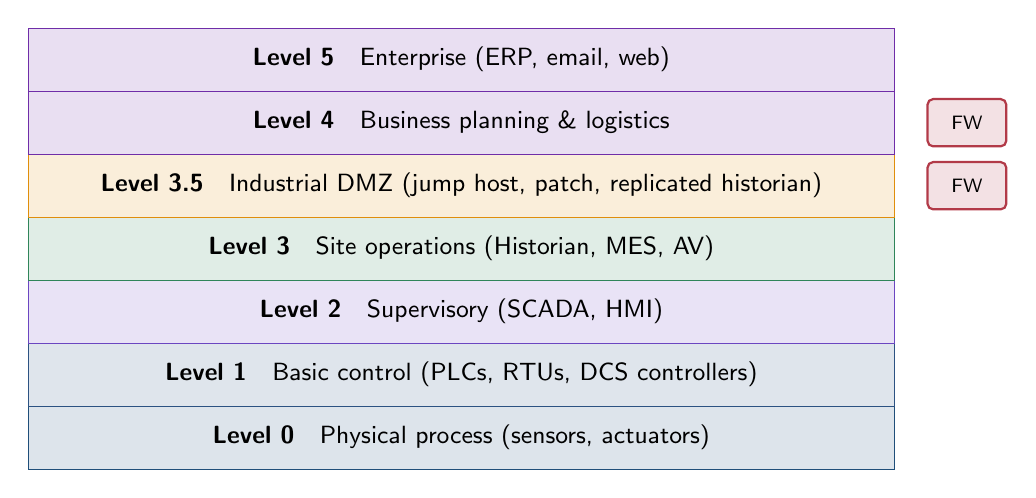
\begin{tikzpicture}[y=0.8cm]
  \foreach \y/\lvl/\desc/\col in {
    0/0/{Physical process (sensors, actuators)}/isOT,
    1/1/{Basic control (PLCs, RTUs, DCS controllers)}/isPLC,
    2/2/{Supervisory (SCADA, HMI)}/isSCADA,
    3/3/{Site operations (Historian, MES, AV)}/isHMI,
    4/{3.5}/{Industrial DMZ (jump host, patch, replicated historian)}/isAccent,
    5/4/{Business planning \& logistics}/isIT,
    6/5/{Enterprise (ERP, email, web)}/isIT}{
    \node[level, fill=\col!15, draw=\col, anchor=west, minimum width=110mm] (L\y) at (0, \y) {\textbf{Level \lvl}\quad \desc};
  }
  \node[firewall, right=4mm of L4, minimum height=6mm, minimum width=10mm, font=\scriptsize] (fw1) {FW};
  \node[firewall, right=4mm of L5, minimum height=6mm, minimum width=10mm, font=\scriptsize] (fw2) {FW};
\end{tikzpicture}
\end{frame}

\begin{frame}{Why an Industrial DMZ?}
\centering
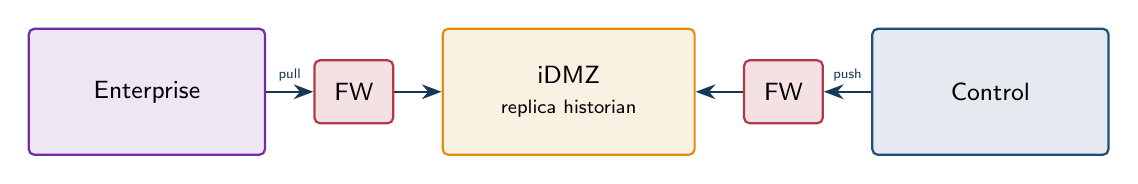
\begin{tikzpicture}[node distance=6mm]
  \node[isbox, fill=isIT!12, draw=isIT, minimum width=30mm, minimum height=16mm] (it) {Enterprise};
  \node[firewall, right=of it, minimum width=10mm] (fw1) {FW};
  \node[isbox, fill=isAccent!12, draw=isAccent, minimum width=32mm, minimum height=16mm, right=of fw1, align=center, font=\small] (dmz) {iDMZ\\\scriptsize replica historian};
  \node[firewall, right=of dmz, minimum width=10mm] (fw2) {FW};
  \node[isbox, fill=isOT!12, draw=isOT, minimum width=30mm, minimum height=16mm, right=of fw2] (ot) {Control};
  \draw[flow] (ot) -- node[above, font=\tiny] {push} (fw2);
  \draw[flow] (fw2) -- (dmz);
  \draw[flow] (it) -- node[above, font=\tiny] {pull} (fw1);
  \draw[flow] (fw1) -- (dmz);
\end{tikzpicture}
\par\vspace{2mm}
\begin{importantbox}{Iron rule}
\textbf{No direct path} between IT and OT. Data \emph{lands} in the DMZ; consumers \emph{pull} from there.
\end{importantbox}
\end{frame}

\section{Topologies}

\begin{frame}{Plant-Floor Topologies}
\centering
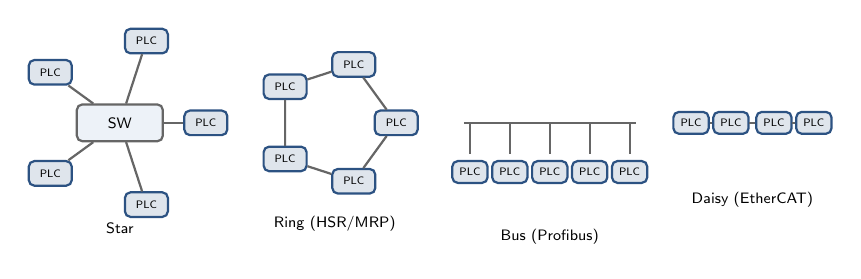
\begin{tikzpicture}[node distance=6mm, scale=0.78, transform shape]
  % star
  \begin{scope}[shift={(0,0)}]
    \node[switch] (s) at (0,0) {SW};
    \foreach \a in {0,72,144,216,288}{\node[plc, minimum width=7mm, minimum height=4mm, font=\tiny] (n\a) at (\a:1.4) {PLC}; \draw[netline] (s)--(n\a);}
    \node[font=\scriptsize, below=12mm of s] {Star};
  \end{scope}
  % ring
  \begin{scope}[shift={(3.5,0)}]
    \foreach \a/\i in {0/A,72/B,144/C,216/D,288/E}{
      \node[plc, minimum width=7mm, minimum height=4mm, font=\tiny] (r\i) at (\a:1.0) {PLC};
    }
    \draw[netline] (rA)--(rB)--(rC)--(rD)--(rE)--(rA);
    \node[font=\scriptsize, below=14mm of {(0,0)}] {Ring (HSR/MRP)};
  \end{scope}
  % bus
  \begin{scope}[shift={(7,0)}]
    \draw[netline] (-1.4,0) -- (1.4,0);
    \foreach \x in {-1.3,-0.65,0,0.65,1.3}{
      \draw[netline] (\x,0) -- (\x,-0.5);
      \node[plc, minimum width=4mm, minimum height=3mm, font=\tiny] at (\x,-0.8) {PLC};
    }
    \node[font=\scriptsize, below=16mm of {(0,0)}] {Bus (Profibus)};
  \end{scope}
  % daisy
  \begin{scope}[shift={(10.3,0)}]
    \foreach \x/\i in {-1.0/1,-0.35/2,0.35/3,1.0/4}{
      \node[plc, minimum width=5mm, minimum height=3mm, font=\tiny] (d\i) at (\x,0) {PLC};
    }
    \draw[netline] (d1)--(d2)--(d3)--(d4);
    \node[font=\scriptsize, below=10mm of {(0,0)}] {Daisy (EtherCAT)};
  \end{scope}
\end{tikzpicture}
\par\vspace{2mm}
\begin{notebox}{Driver}
Topology choice in OT is driven by \textbf{determinism} and \textbf{availability}, not security.
\end{notebox}
\end{frame}

\section{Zones and Conduits}

\begin{frame}{Zones and Conduits (IEC 62443)}
\centering
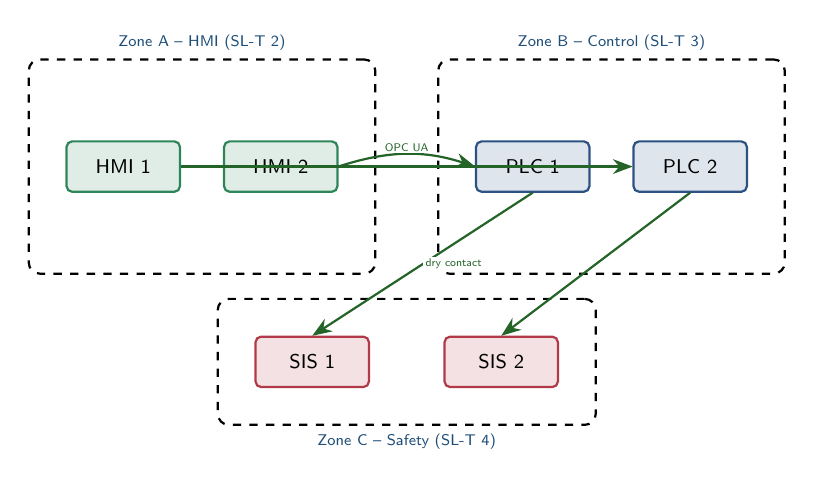
\begin{tikzpicture}[node distance=8mm, scale=0.8, transform shape]
  \begin{scope}[on background layer]
    \node[zone, fit={(0,0) (4.5,2.4)}, label={[font=\scriptsize, color=isOT]above:Zone A -- HMI (SL-T 2)}] {};
    \node[zone, fit={(6.5,0) (11,2.4)}, label={[font=\scriptsize, color=isOT]above:Zone B -- Control (SL-T 3)}] {};
    \node[zone, fit={(3,-2.4) (8,-1.4)}, label={[font=\scriptsize, color=isOT]below:Zone C -- Safety (SL-T 4)}] {};
  \end{scope}
  \node[hmi] (h1) at (1.0,1.2) {HMI 1};
  \node[hmi] (h2) at (3.5,1.2) {HMI 2};
  \node[plc] (p1) at (7.5,1.2) {PLC 1};
  \node[plc] (p2) at (10.0,1.2) {PLC 2};
  \node[plc, fill=isAttack!15, draw=isAttack] (s1) at (4.0,-1.9) {SIS 1};
  \node[plc, fill=isAttack!15, draw=isAttack] (s2) at (7.0,-1.9) {SIS 2};
  \draw[conduit] (h2.east) to[bend left=18] node[above, font=\tiny, sloped, fill=white, inner sep=1pt] {OPC UA} (p1.west);
  \draw[conduit] (h1.east) -- (p2.west);
  \draw[conduit] (p1.south) -- node[right, font=\tiny, fill=white, inner sep=1pt] {dry contact} (s1.north);
  \draw[conduit] (p2.south) -- (s2.north);
\end{tikzpicture}
\par\vspace{1mm}
{\footnotesize Zones group assets with similar security needs; conduits are the controlled channels between them.}
\end{frame}

\begin{frame}{Industrial Firewalls}
\centering
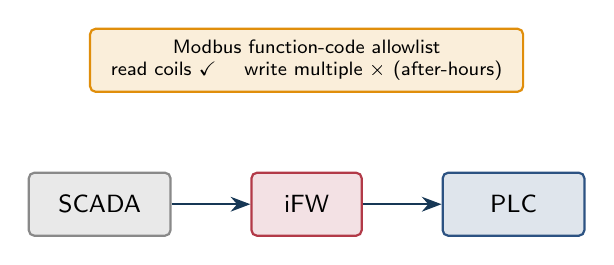
\begin{tikzpicture}[node distance=10mm]
  \node[server] (s) {SCADA};
  \node[firewall, right=of s, minimum width=14mm] (fw) {iFW};
  \node[plc, right=of fw] (p) {PLC};
  \node[isbox, fill=isAccent!15, draw=isAccent, above=of fw, font=\scriptsize, align=center, minimum width=55mm]
    {Modbus function-code allowlist\\read coils \checkmark{} \quad write multiple \texttimes{} (after-hours)};
  \draw[flow] (s) -- (fw);
  \draw[flow] (fw) -- (p);
\end{tikzpicture}
\par\vspace{3mm}
\footnotesize Industrial firewalls do stateful inspection \emph{and} ICS protocol parsing. Often deployed transparently.
\end{frame}

\begin{frame}{Data Diode -- One-Way Egress}
\centering
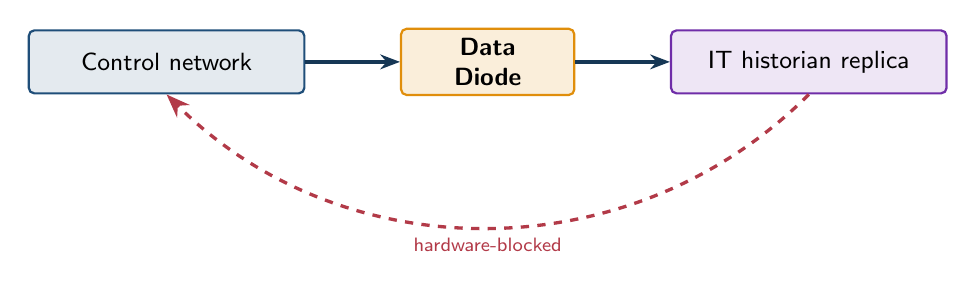
\begin{tikzpicture}[node distance=12mm]
  \node[isbox, fill=isOT!12, draw=isOT, minimum width=35mm] (ctrl) {Control network};
  \node[isbox, fill=isAccent!15, draw=isAccent, right=of ctrl, minimum width=22mm, font=\small\bfseries] (diode) {Data\\Diode};
  \node[isbox, fill=isIT!12, draw=isIT, right=of diode, minimum width=35mm] (it) {IT historian replica};
  \draw[flow, very thick] (ctrl) -- (diode);
  \draw[flow, very thick] (diode) -- (it);
  \draw[-{Stealth[length=3mm]}, very thick, isAttack, dashed] (it.south) to[bend left=45] node[below, font=\scriptsize] {hardware-blocked} (ctrl.south);
\end{tikzpicture}
\par\vspace{2mm}
\footnotesize Physical fibre layout enforces the direction. Useful for safety-critical data egress.
\end{frame}

\begin{frame}{Wireless in OT}
\centering
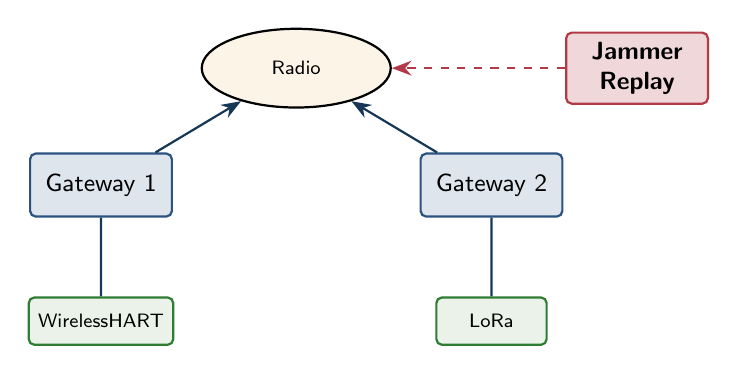
\begin{tikzpicture}[node distance=10mm]
  \node[inetnode, fill=isAccent!10] (rf) {Radio};
  \node[plc, below left=of rf] (g1) {Gateway 1};
  \node[plc, below right=of rf] (g2) {Gateway 2};
  \node[sensor, below=of g1] (s1) {WirelessHART};
  \node[sensor, below=of g2] (s2) {LoRa};
  \node[attacker, right=22mm of rf, align=center] (atk) {Jammer\\ Replay};
  \draw[flow] (s1) -- (g1) -- (rf);
  \draw[flow] (s2) -- (g2) -- (rf);
  \draw[attack] (atk) -- (rf);
\end{tikzpicture}
\par\vspace{2mm}
\footnotesize Convenience vs.\ attack surface. Never put safety-critical loops over uncontrolled wireless.
\end{frame}

\begin{frame}{VLANs in OT -- Useful, Not Sufficient}
\centering
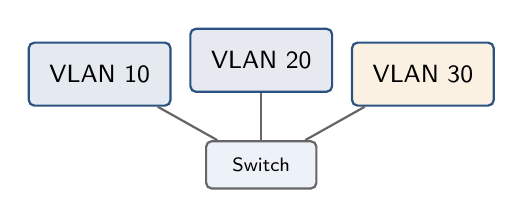
\begin{tikzpicture}[node distance=6mm]
  \node[switch] (sw) {Switch};
  \node[plc, fill=isOT!12, above left=of sw] (v1) {VLAN 10};
  \node[plc, fill=isPLC!12, above=of sw] (v2) {VLAN 20};
  \node[plc, fill=isAccent!12, above right=of sw] (v3) {VLAN 30};
  \foreach \n in {v1,v2,v3}{\draw[netline] (\n)--(sw);}
\end{tikzpicture}
\vspace{2mm}
\begin{warnbox}{VLAN hopping is a real attack}
A misconfigured trunk port (DTP enabled, native VLAN guessed) lets an attacker hop between VLANs. Use VLANs for organisation; require a routed firewall for security boundaries.
\end{warnbox}
\end{frame}

\begin{frame}{NAT in OT -- When Not to Use}
\centering

\begin{tikzpicture}[node distance=8mm]
  \node[isbox, fill=isIT!12, draw=isIT, minimum width=40mm] (it) {IT 10.0.0.0/8};
  \node[firewall, right=of it, minimum width=14mm] (nat) {NAT};
  \node[isbox, fill=isOT!12, draw=isOT, minimum width=40mm, right=of nat] (ot) {OT 192.168.10.0/24};
  \draw[flow] (it) -- (nat) -- (ot);
\end{tikzpicture}
\vspace{2mm}
\begin{importantbox}{NAT hides, it does not protect}
NAT breaks end-to-end addressability -- useful for legacy duplicate networks, harmful for incident analysis. Prefer routed, segmented design with explicit firewall rules.
\end{importantbox}
\end{frame}

\begin{frame}{Time Synchronisation in OT}
\centering
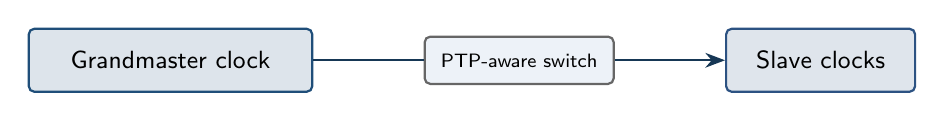
\begin{tikzpicture}[node distance=10mm]
  \node[isbox, fill=isOT!15, draw=isOT, minimum width=36mm, font=\small] (gm) {Grandmaster clock};
  \node[switch, right=14mm of gm, minimum width=24mm] (sw) {PTP-aware switch};
  \node[plc, right=14mm of sw, minimum width=24mm] (s) {Slave clocks};
  \draw[flow] (gm) -- (sw) -- (s);
\end{tikzpicture}
\vspace{2mm}
\begin{notebox}{Why it matters for security}
Without synchronised clocks, alarm logs and PCAPs are useless in forensics. PTP (IEEE 1588) gives sub-microsecond accuracy on the plant floor; NTP is enough for L3+.
\end{notebox}
\end{frame}

\begin{frame}{SPAN, TAP, and Visibility}
\centering
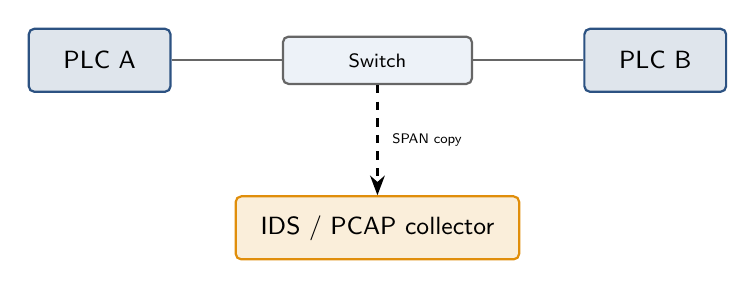
\begin{tikzpicture}[node distance=8mm]
  \node[switch, minimum width=24mm] (sw) {Switch};
  \node[plc, left=14mm of sw] (a) {PLC A};
  \node[plc, right=14mm of sw] (b) {PLC B};
  \node[isbox, fill=isAccent!15, draw=isAccent, below=14mm of sw, minimum width=36mm, font=\small] (ids) {IDS / PCAP collector};
  \draw[netline] (a) -- (sw); \draw[netline] (sw) -- (b);
  \draw[-{Stealth[length=2.5mm]}, dashed, thick] (sw) -- node[right=3pt, font=\tiny, fill=white, inner sep=2pt]{SPAN copy} (ids);
\end{tikzpicture}
\vspace{2mm}
\begin{notebox}{SPAN vs hardware TAP}
SPAN can drop packets under load and lets the switch see your collector. A hardware TAP is read-only by construction -- preferred for high-fidelity capture.
\end{notebox}
\end{frame}

\begin{frame}{Wireless Generations on the Plant}
\centering
\renewcommand{\arraystretch}{1.2}
\footnotesize
\begin{tabular}{|p{3cm}|p{2.6cm}|p{2.4cm}|p{3.8cm}|}
\hline
\rowcolor{slidePanel}
\textbf{Tech} & \textbf{Latency} & \textbf{Range} & \textbf{Typical use} \\
\hline
Wi-Fi 6 / 6E   & 1--10 ms & 10--100 m & Mobile HMI, video \\
WirelessHART   & 250 ms   & 100 m     & Process sensors \\
ISA-100.11a    & 250 ms   & 100 m     & Process sensors \\
LoRaWAN        & seconds  & km        & Building automation \\
NB-IoT / LTE-M & seconds  & km        & Remote telemetry \\
Private 5G     & 1 ms     & 100--500 m & High-density factory \\
\hline
\end{tabular}
\end{frame}

\begin{frame}{Summary -- Section \sectionNumber}
\begin{takeawaybox}{What to remember from this section}
\begin{itemize}\setlength{\itemsep}{2pt}
  \item The Purdue model groups assets into layers; firewalls separate the layers.
  \item The Industrial DMZ brokers all traffic between corporate IT and the plant.
  \item Zones and conduits give a structured language for IEC 62443 design.
  \item Hardware mediation (diodes, gateways) protects the most sensitive flows.
\end{itemize}
\end{takeawaybox}
\end{frame}

\referencesframe{
  \item Williams, T.J. \emph{The Purdue Enterprise Reference Architecture}, Computers in Industry, 1994.
  \item ANSI/ISA-95 (IEC 62264). \emph{Enterprise-Control System Integration}.
  \item IEC 62443-3-2:2020. \emph{Security risk assessment for system design} (zones \& conduits).
  \item IEC 62439-3:2021. \emph{High Availability Seamless Redundancy (HSR) and Parallel Redundancy Protocol (PRP)}.
  \item IEEE 1588-2019. \emph{Precision Time Protocol (PTP)}.
  \item IEC 62591:2016. \emph{WirelessHART}.
  \item IEC 62734:2014. \emph{ISA-100.11a wireless system for industrial automation}.
  \item Idaho National Lab. \emph{Recommended Practice: Improving Industrial Control System Cybersecurity with Defense-in-Depth Strategies}, 2016.
  \item CISA. \emph{Securing Network Infrastructure Devices}, 2018.
  \item Stouffer, K. et al. \emph{NIST SP 800-82 Rev.\,3 -- Guide to OT Security}, Sep 2023.
}

\closingframe

\end{document}
